\section{Modular Coding and Linking}

\begin{concept}{Modular Programming Overview}\\
Program code is divided into modules with:
\begin{itemize}
  \item Each source file compiled into separate object file
  \item All object files linked into single executable
  \item Clear interfaces between modules
\end{itemize}

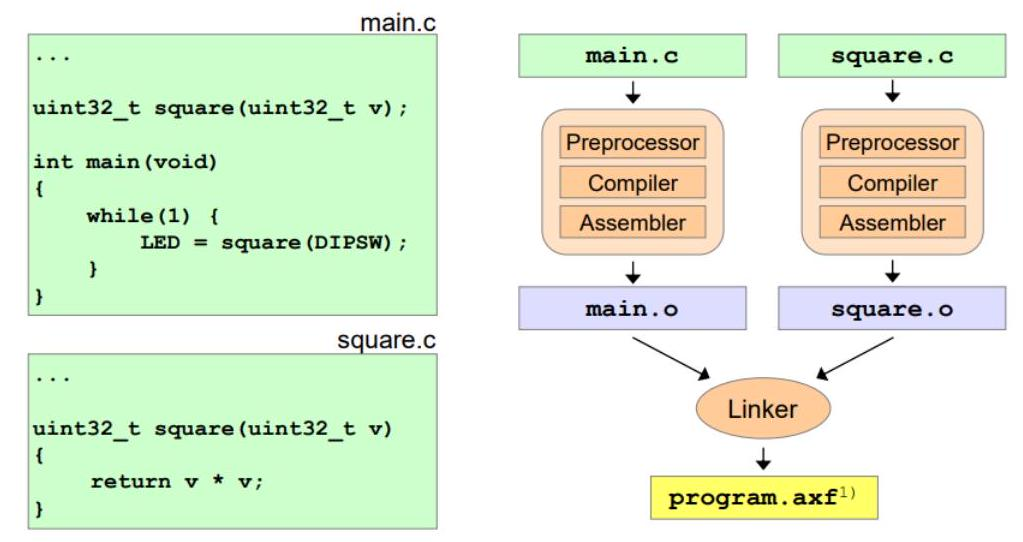
\includegraphics[width=\linewidth]{images/2024_12_29_79e6b22f503fb7b4f718g-10(2)}
\end{concept}

\begin{definition}{Benefits of Modular Programming}\\
Key advantages:
\begin{itemize}
  \item \textbf{Team Development}:
    \begin{itemize}
      \item Multiple developers working on same codebase
      \item Clear ownership of modules
    \end{itemize}
  \item \textbf{Code Organization}:
    \begin{itemize}
      \item Logical partitioning of functionality
      \item Easier code reuse
    \end{itemize}
  \item \textbf{Development Efficiency}:
    \begin{itemize}
      \item Individual module testing
      \item Faster compilation (only changed modules)
      \item Reusable library creation
    \end{itemize}
  \item \textbf{Language Integration}:
    \begin{itemize}
      \item Mix C and assembly modules
      \item Language-specific optimizations
    \end{itemize}
\end{itemize}
\end{definition}

\begin{definition}{Module Linkage}\\
Keywords for controlling module interfaces:
\begin{itemize}
  \item \textbf{EXPORT}: Make symbol available to other modules
  \item \textbf{IMPORT}: Use symbol from another module
  \item Internal symbols: Neither IMPORT nor EXPORT
\end{itemize}

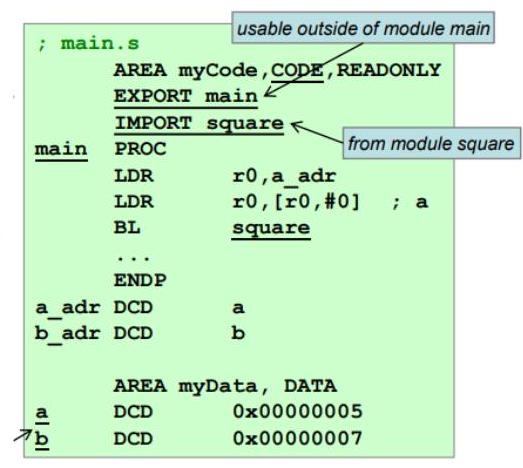
\includegraphics[width=\linewidth]{images/2024_12_29_79e6b22f503fb7b4f718g-10(1)}
\end{definition}

\begin{definition}{Object Files}\\
ELF format contains:
\begin{itemize}
  \item \textbf{Code Section}:
    \begin{itemize}
      \item Program code and constants
      \item Based at address 0x0
    \end{itemize}
  \item \textbf{Data Section}:
    \begin{itemize}
      \item Global variables
      \item Based at address 0x0
    \end{itemize}
  \item \textbf{Symbol Table}:
    \begin{itemize}
      \item All symbols and their attributes
      \item Global/local status
      \item References to external symbols
    \end{itemize}
  \item \textbf{Relocation Table}:
    \begin{itemize}
      \item Instructions for adjusting addresses
      \item Applied during linking process
    \end{itemize}
\end{itemize}
\end{definition}

\begin{concept}{Linker Operation}\\
Main tasks:
\begin{itemize}
  \item Merge code sections from all objects
  \item Merge data sections from all objects
  \item Resolve symbol references between modules
  \item Relocate addresses to final positions
\end{itemize}

Output is ARM Executable File (AXF):

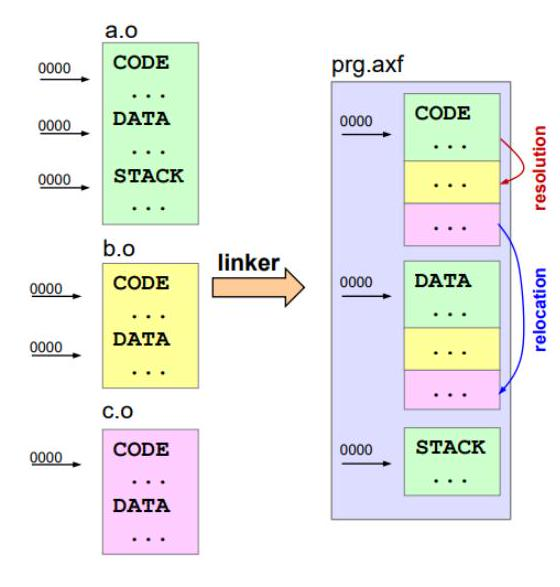
\includegraphics[width=\linewidth]{images/2024_12_29_79e6b22f503fb7b4f718g-10}
\end{concept}

\begin{example2}{Module Interface Example}
\begin{lstlisting}[language=armasm, style=basesmol]
    ; Module A - Defining function
    AREA myCode, CODE, READONLY
    EXPORT myFunction    ; Make available externally
myFunction
    PUSH    {LR}
    ; function code here
    POP     {PC}
    
    ; Module B - Using function
    AREA myCode, CODE, READONLY
    IMPORT myFunction    ; Use external function
    
    BL      myFunction   ; Call the function
\end{lstlisting}
\end{example2}

\begin{KR}{Creating Modular Programs}\\
Steps for modular development:
\begin{enumerate}
  \item Design module structure:
    \begin{itemize}
      \item Identify clear boundaries
      \item Define interfaces
    \end{itemize}
  \item Create individual modules:
    \begin{itemize}
      \item Declare IMPORT/EXPORT
      \item Implement functionality
    \end{itemize}
  \item Compile modules separately
  \item Link modules:
    \begin{itemize}
      \item Resolve references
      \item Create executable
    \end{itemize}
  \item Test integrated system
\end{enumerate}
\end{KR}